\section{Top quark physics} % (fold)
\label{sec:top_quark_physics}

The top quark was first seen by the CDF and D0 experiments at the Tevatron in 1994, with the discovery being published in 1995.
It is the most massive particle in the SM to date, at 172.5\GeV{}.
The large mass means that the lifetime of the top quark is very short at $\sim5\ten{-25}\s$\,\cite{PDG}.
In fact, it is shorter than the typical time it takes for a quark to hadronise, such that it is possible for the bare quark properties to be measured directly.

Now, at the LHC, more top quarks are being produced than ever before, leading to a vast array of measurements being performed, such as precision measurements of the \SM{}, searches for rare \SM{} processes and searches for possible new physics present in their decays.
Not only is top quark physics important in direct searches for new physics, it is often the process which forms the largest background in other searches for particles beyond the \SM{}.
Therefore, it is crucial to know the production cross section of the top quark as precisely as possible.
The precise top quark production cross section measurements can also uniquely be used to directly probe the $V_{tb}$ element of the CKM matrix ($V_{tb} >> V_{ts} > V_{td}$), to set constraints on the gluon PDF and to measure the top Yukawa coupling strength.


\subsection{Top quark production} % (fold)
\label{sub:top_quark_production}

Protons are made up of three valence quarks (\uquark{}\uquark{}\dquark{}), confined by gluons. 
At higher energies, the gluon multiplicity increases, as well as the number of pair-produced \qqbar{} pairs, known as sea quarks.
This means that it is much more probable that an interaction will occur from collisions between gluons or non-valence quarks.
Top quark production at the LHC at \com{} proceeds primarily via \ttbar{} pair-production, where $\sim90\%$ is from gluon-gluon fusion. 
The further $\sim10\%$ comes from quark-anti-quark annihilation and is shown in Fig\,\ref{fig:feyn-eg}. 
The top quark can also be produced singly or as a quadruplet, as shown in Figs\,\ref{fig:feyn-t} and \ref{fig:feyn-tttt}.
% Measurements of single top production are especially interesting as the cross section is directly proportional to the $|V_{tb}|$ matrix element (assuming $|V_{tb}| >> |V_{ts}| > |V_{td}|$)
% Add Vtb and top spin?
\begin{figure}[h!]
	\centering
	\begin{subfigure}{.32\textwidth}
		\centering
		\begin{tikzpicture}
		\begin{feynman}
			\vertex (A);
			\vertex [above left=0.75cm and 1.5cm of A] (ai) {\(\overline{q}'\)};
			\vertex [below left=0.75cm and 1.5cm of A] (aii) {\(q\)};

			\vertex [right=1.5cm of A] (B);
			\vertex [above right=0.75cm and 1.5cm of B] (bi) {\(t\)};
			\vertex [below right=0.75cm and 1.5cm of B] (bii) {\(\overline{b}\)};

			\diagram*{
			(ai) -- [anti fermion] (A),
			(aii) -- [fermion] (A),
			(A) -- [boson, edge label=\(W^{+}\)] (B),
			(B) -- [fermion] (bi),
			(B) -- [anti fermion] (bii),
			};
		\end{feynman}
		\end{tikzpicture}
	\end{subfigure}
	\begin{subfigure}{.32\textwidth}
		\centering
		\begin{tikzpicture}
		\begin{feynman}
			\vertex [black](i1){\(q\)};
			\vertex [black,right=1.5cm of i1](a);
			\vertex [black,above right=0.75cm and 1.5cm of a](f1){\(q'\)};
			\vertex [black,below right=0.75cm and 1.5cm of a](b);
			\vertex [black,right=1.5cm of b](f2){\(t\)};
			\vertex [black,below=1.5cm of i1](i2){\(g\)};
			\vertex [black,right=1.5cm of i2](c);
			\vertex [black,below right=0.75cm and 1.5cm of c] (f3){\(\overline{b}\)};

			\diagram* {
			(i1) -- [black,fermion] (a) -- [black,fermion] (f1),
			(a) -- [black,boson, edge label=\(W^{+}\)] (b),
			(i2) -- [black,gluon] (c),
			(c) -- [black,fermion] (b),
			(b) -- [black,fermion] (f2),
			(c) -- [black,anti fermion] (f3),
			};
		\end{feynman}
		\end{tikzpicture}
	\end{subfigure}
	\begin{subfigure}{.32\textwidth}
		\centering
		\begin{tikzpicture}
		\begin{feynman}
			\vertex [black](i1){\(g\)};
			\vertex [black,right=1.5cm of i1](a);
			\vertex [black,above right=0.75cm and 1.5cm of a](f1){\(t\)};
			\vertex [black,below right=0.75cm and 1.5cm of a](b);
			\vertex [black,right=1.5cm of b](f2){\(W^{-}\)};
			\vertex [black,below=1.5cm of i1](i2){\(g\)};
			\vertex [black,right=1.5cm of i2](c);
			\vertex [black,below right=0.75cm and 1.5cm of c] (f3){\(\overline{b}\)};

			\diagram* {
			(i1) -- [black,gluon] (a)
			(a) -- [black,fermion] (f1),
			(a) -- [black,anti fermion] (b),
			(b) -- [black,boson] (f2),
			(i2) -- [black,gluon] (c),
			(c) -- [black,fermion] (b),
			(c) -- [black,anti fermion] (f3),
			};
		\end{feynman}
		\end{tikzpicture}
	\end{subfigure}
	\caption[Feynman diagrams for the production of single top quarks. On the left, via the s-channel, in the middle via the t-channel and on the right via the tW channel.]{Feynman diagrams for the production of single top quarks. On the left, via the s-channel, in the middle via the t-channel and on the right via the tW channel. }
	\label{fig:feyn-t}
\end{figure}
\begin{figure}[h!]
	\centering
	\begin{subfigure}{.49\textwidth}
		\centering
		\begin{tikzpicture}
		\begin{feynman}
			\vertex [black](i1){\(g\)};
			\vertex [black,right=1.5cm of i1](a);
			\vertex [black,above right=0.75cm and 1.5cm of a](f1){\(t\)};
			\vertex [black,below right=0.75cm and 1.5cm of a](b);
			\vertex [black,right=1.5cm of b](f2);
			\vertex [black,above right=0.75cm and 1.5cm of f2](f2a){\(t\)};
			\vertex [black,below right=0.75cm and 1.5cm of f2](f2b){\(\overline{t}\)};
			\vertex [black,below=1.5cm of i1](i2){\(g\)};
			\vertex [black,right=1.5cm of i2](c);
			\vertex [black,below right=0.75cm and 1.5cm of c] (f3){\(\overline{t}\)};

			\diagram* {
			(i1) -- [black,gluon] (a)
			(a) -- [black,fermion] (f1),
			(a) -- [black,anti fermion] (b),
			(b) -- [black,gluon] (f2),
			(f2) -- [black,fermion] (f2a),
			(f2) -- [black,anti fermion] (f2b),
			(i2) -- [black,gluon] (c),
			(c) -- [black,fermion] (b),
			(c) -- [black,anti fermion] (f3),
			};
		\end{feynman}
		\end{tikzpicture}
	\end{subfigure}
	\begin{subfigure}{.49\textwidth}
		\centering
		\begin{tikzpicture}
		\begin{feynman}
			\vertex [black](i1){\(g\)};
			\vertex [black,right=1.5cm of i1](a);
			\vertex [black,above right=0.75cm and 1.5cm of a](f1){\(\overline{t}\)};
			\vertex [black,below right=0.75cm and 1.5cm of a](c);
			\vertex [black,above right=0.75cm and 1.5cm of b](f2){\(t\)};

			\vertex [black,below=2.5cm of i1](i2){\(g\)};
			\vertex [black,right=1.5cm of i2](b);
			\vertex [black,above right=0.75cm and 1.5cm of b](d);
			\vertex [black,below right=0.75cm and 1.5cm of b](f3){\(t\)};
			\vertex [black,below right=0.75cm and 1.5cm of d](f4){\(\overline{t}\)};

			\diagram* {
			(i1) -- [black,gluon] (a)
			(a) -- [black,anti fermion] (f1),
			(a) -- [black,fermion] (c),
			(c) -- [black,fermion] (f2),
			
			(c) -- [black,gluon] (d),

			(i2) -- [black,gluon] (b)
			(b) -- [black,fermion] (f3),
			(b) -- [black,anti fermion] (d),
			(d) -- [black,anti fermion] (f4),
			};
		\end{feynman}
		\end{tikzpicture}
	\end{subfigure}
	\caption[Feynman diagrams for the production of four top quarks. The mediating boson is predominantly a gluon, however photons, \Zboson{} bosons and \Hboson{} bosons can also mediate.]{Feynman diagrams for the production of four top quarks. The mediating boson is predominantly a gluon, however photons, \Zboson{} bosons and \Hboson{} bosons can also mediate. }
	\label{fig:feyn-tttt}
\end{figure}

The production cross section for the interaction $\sigma_{pp\to\ttbar{}}$, is predicted by the convolution of the partonic cross section $\hat{\sigma}_{\ttbar{}}$ derived directly from the Feynman diagrams and the \textit{parton distribution functions} (PDFs) of the incident protons $f(x, Q^{2})$, summed over all possible parton flavours.
This is given by
\begin{equation}
\label{eq:pdf}
	\sigma_{pp\to\ttbar{}} = \sum_{a, b}\int_{0}^{1}f(x_{a}, Q^{2})dx_{a}\,\,.\,\int_{0}^{1}f(x_{b}, Q^{2})dx_{b}\,\,.\,\,\hat{\sigma}_{ab\to\ttbar{}}.
\end{equation}
The PDF is defined as the number density of a parton carrying a fraction, $x$, of the protons total momentum in the longitudinal direction at the energy scale being probed, $Q$.

The PDFs are measured from global fits to many different data measurements and sources, such as measurements of deep inelastic scattering, Drell-Yan production and inclusive jet production, from experiments such as HERA, D0 and CMS.
The PDF is calculated at some arbitrary $Q^{2} = Q^{2}_{0}$, which is taken as 1\GeV{} by the $\mathrm{NNPDF}$ collaboration in the $\mathrm{NNPDF3.1}$ pdf set.
This is then evolved through the DGLAP equations to higher energy scales.
The $xf(x, Q^{2})$ distributions for the $\mathrm{NNPDF3.1}$ pdf set at $Q^{2} = 10\GeVsq$ and $Q^{2} = 10^{4}\GeVsq$ set are displayed in Fig.\,\ref{fig:pdf}.
\begin{figure}[htpb]
	\centering
	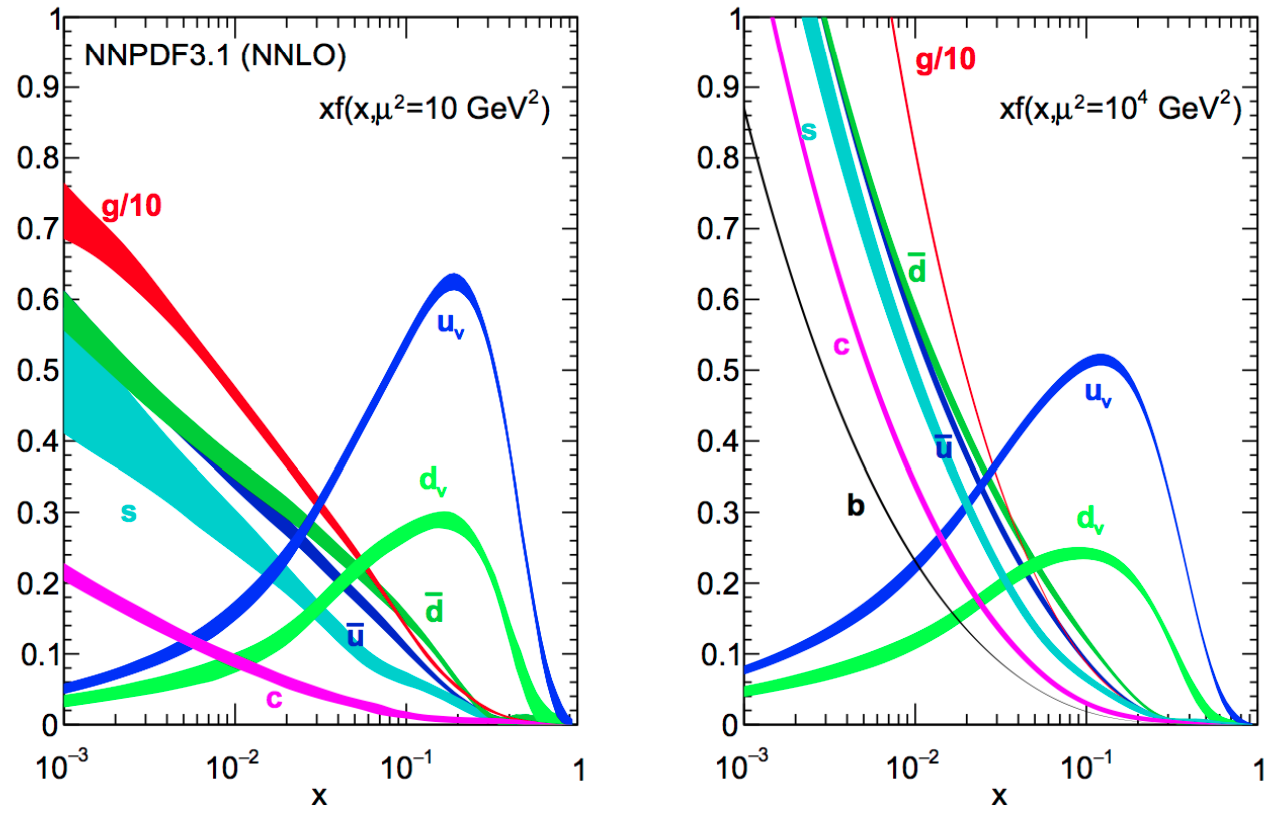
\includegraphics[width=0.9\textwidth]{Figures/PDF}
	\caption[The parton distribution function of the proton scaled by the fraction of momentum carried by the parton, $xf(x, Q^2)$ with respect to the fraction of momentum carried by the parton. The left panel shows the distributions with respect to a lower energy scale and the right panel with respect to a higher energy scale.]{ The parton distribution function of the proton scaled by the fraction of momentum carried by the parton, $xf(x, Q^2)$ with respect to the fraction of momentum carried by the parton. The left panel shows the distributions with respect to a lower energy scale and the right panel with respect to a higher energy scale\,\cite{NNPDF3p1}. }
	\label{fig:pdf}
\end{figure}
When moving from low to high $Q^{2}$ values, it is clearly seen that more of the protons momentum is carried by an increasing number of non-valence partons.

The prediction of the inclusive \ttbar{} cross section from proton-proton collisions is shown in Fig.\,\ref{fig:incttbar}, together with current experimental measurements. 
Also shown is the prediction from proton-anti-proton collisions.
At \com{}, the inclusive \ttbar{} production cross section was calculated to be $831.8^{+19.8}_{-29.2}(\text{scale})\pm35.1(\text{PDF}+\alpS)\pb$\,\cite{TOPpp}.
% TODO ADD MORE?
\begin{figure}[htpb]
	\centering
	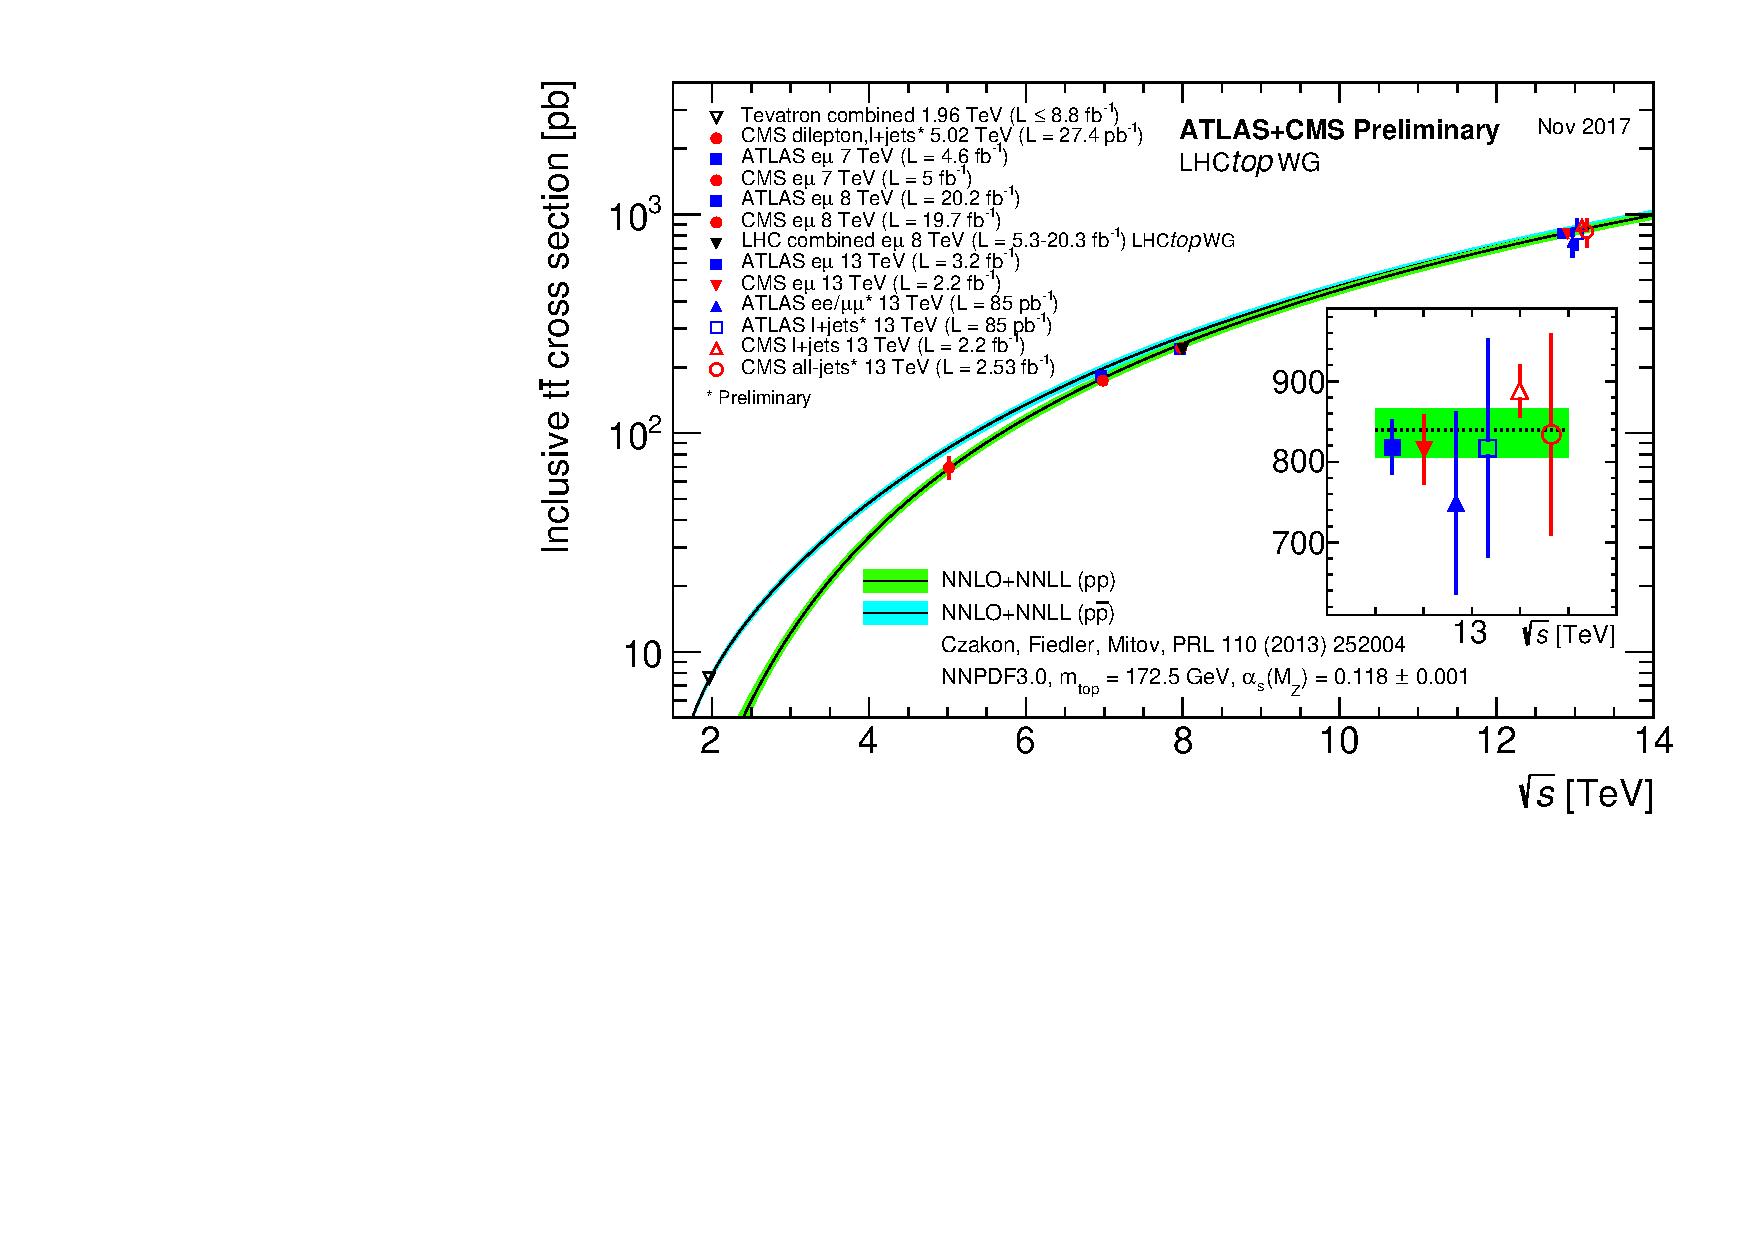
\includegraphics[width=0.9\textwidth]{Figures/tt_curve_sqrts_cms}
	\caption[The inclusive \ttbar cross section, measured by both ATLAS and CMS in different decay channels at \sqrts{} = 5, 7, 8 and 13\TeV{}. Also shown is the most precise theoretical prediction to date.]{ The inclusive \ttbar cross section, measured by both ATLAS and CMS in different decay channels at \sqrts{} = 5, 7, 8 and 13\TeV{}. Also shown is the most precise theoretical prediction to date\,\cite{LHCTopWG_Plots} }
	\label{fig:incttbar}
\end{figure}
% subsection top_quark_production (end)

\subsection{Top quark decay} % (fold)
\label{sub:top_quark_decay}

The top quark will decay 99.8\%\,\cite{PDG} of the time to a \bquark{} quark and \Wboson{} boson.
The \Wboson{} boson then subsequently decays either into \qpqbar{} pair (hadronic) or a \lepton{}\neutrinobar{} pair (leptonic).
In the case of \ttbar{} production, this leads to three classes of final states, the first where both \Wboson{} bosons decay leptonically, the second where both decay  hadronically and lastly where one decays leptonically and the other hadronically.
These are known as the \textit{dilepton}, \textit{all-hadronic} and \textit{single lepton} decay channels respectively.
The probability of decaying to a specific final state (\textit{branching ratio}) is approximately $10\%$ for the dilepton channel and $45\%$ for the hadronic and single lepton channels.
% W->(ud*3, cs*3, enu, munu, taunu) us cd suppressed

Each final state category has merits and drawbacks. 
The dilepton final state provides the most clean experimental signature, however this comes at the cost of a reduced branching ratio.
It is aslo difficult to fully reconstruct the whole process as both neutrinos contribute to the single source of missing transverse momentum.
The all-hadronic final state in comparison has a large branching ratio, but the large number of jets in the final state leads to significant backgrounds from multijet QCD production.
While the all-hadronic final state is difficult at lower collision energies, it gains in sensitivity when analysed at high collision energies.
This is because the decay products of the top quark collimate and merge into a single jet, which is able to be tagged as coming from a top quark, through jet-substructure techniques.
Finally the single lepton decay channel has a large branching ratio, but with much reduced backgrounds with respect to the all-hadronic final state. The final state in which a tau particle is produced is often neglected however, due to the added complexity of reconstructing it.
More details about the reconstruction of particles can be found in Section TODO.
% For this reason \lepton{} will be used to refer to just \electron{} and \muon{}.
% subsection tt_decay (end)

\subsection{Top quark cross section measurements} % (fold)
\label{sub:top_quark_cross_section_measurements}

Figure.\,\ref{fig:incttbar} shows, in addition to the theoretical prediction of the inclusive \ttbar{} production cross section, the corresponding experimental measurements, from both Compact Muon Solenoid (CMS) and A Toriodal Large ApparatuS (ATLAS) at different \sqrts{} in all of the channels previously stated.
At CMS, the inclusive \ttbar{} cross section measurements are performed at 13\TeV{}\,\cite{TOP16005, TOP16006} at 7 and 8 \TeV{}\,\cite{TOP10001, TOP10002, TOP10003, TOP11002, TOP11003, TOP11004, TOP11005, TOP12007, TOP12026, TOP12041, TOP13004, TOP14018} and at 5\TeV{}\,\cite{TOP16023}.
Inclusive cross section measurements have been performed for \ttbar{} production in association with a photon\,\cite{TOP14008}, vector boson\,\cite{TOP17005} and most recently \Hboson{} boson\,\cite{HIG17035}.

Measurements of the \ttbar{} production cross section with respect to some kinematic distribution are known as \textit{differential} cross section measurements.
Differential cross section measurements are especially useful for testing the understanding of state-of-the-art theoretical models.
Ideally, these models should describe \ttbar{} production with respect to all kinematic distributions accurately and for all \sqrts{}.
In practice this is not the case, with the \ttbar{} models being \textit{tuned} to best decribe the kinematic distributions.
A tune is a complete set of parameters describing physics processes within the model, which have been tweaked to best describe differential data distributions.
Figure.\,\ref{fig:8TeVTuning} shows the effect of this tuning on a set of \ttbar{} models, where the new tune is shown in solid and the old in dashed, when compared against the magnitude of the transverse momentum of the hadronically decaying top quark, \ptToph{}, and the additional jet multiplicity.
It is worth noting, that a tune applied to a specific model, may not describe the differential data better than when applied to an another independent model.
The different models behind \ttbar{} production are expained in more detail in Section TODO.
Indeed by changing the tune, it may cause the same model to describe some kinematic distributions to a worse degree.
\begin{figure}[htpb]
	\centering
	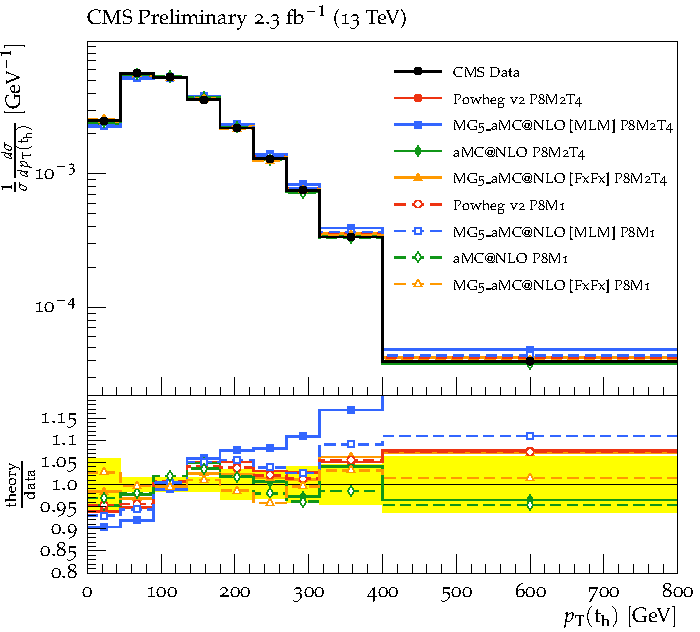
\includegraphics[width=0.49\textwidth]{Figures/TuningEx3}
	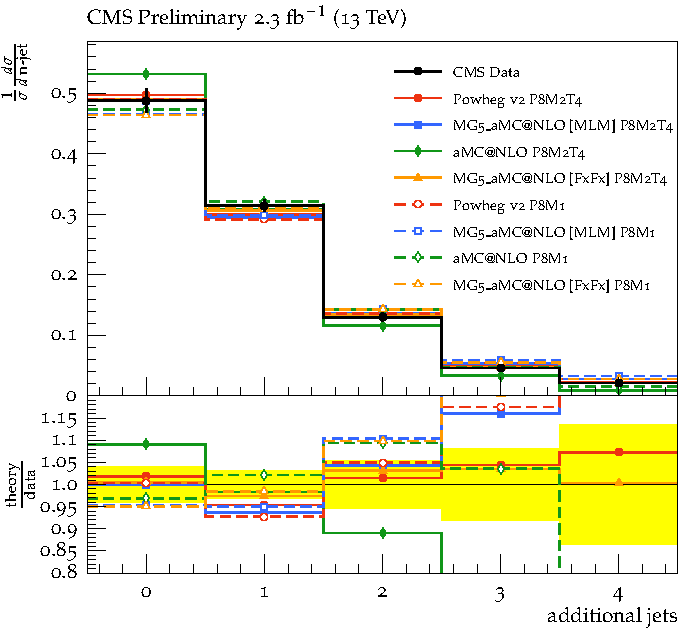
\includegraphics[width=0.49\textwidth]{Figures/TuningEx2}
	\caption[Comparison of different \ttbar{} models with the old \CUETold{} tune and the new \CUET{} tune. The left panel shows the comparison for the distribution of the \pt{} of the hadronically decaying top quark and the right panel for the additional jets distribution.]{ Comparison of different \ttbar{} models with the old \CUETold{} tune and the new \CUET{} tune. The left panel shows the comparison for the distribution of the \pt{} of the hadronically decaying top quark and the right panel for the additional jets distribution\,\cite{TOP16021}. }
	\label{fig:8TeVTuning}
\end{figure}

Differential top quark cross section measurements can be presented to \textit{particle level} where the kinematic distributions are constructed with respect to stable particles in the detector (mean lifetime longer than 30\ps{}).
Alternatively, they can be presented to \textit{parton level}, where the results are extrapolated with respect to the final state partons.
Similarly, the results can be presented in a phase space similar to that accessible by the detector, the \textit{visible phase space} or extrapolated to the \textit{full phase space}.
Measurements that are presented to parton level or that are extrapolated to the full phase space are influenced by large theoretical uncertainties and as such most analyses present measurements to particle level in the visible phase space.
Each measurement performed by the CMS (and ATLAS) experiment are completely complementary to each other and are presented at 7 and 8\TeV{}\,\cite{TOP11013,TOP12028,TOP14012,TOP14013} and at 13\TeV\,\cite{TOP16007,TOP16008,TOP16010,TOP17002}.

This thesis looks at differential cross section measurements as a function of kinematic event variables in the single lepton channel presented to particle level in a visible phase space.
The kinematic event variables are variables which do not require the reconstruction of the complete \ttbar{} system.
The event variables considered are the jet multiplicity, \NJET{}, the scalar sum of the jet \pt{}, \HT{}, the scalar sum of the \pt{} of all particles, \ST{}, the magnitudes of the transverse momentum imbalance, \ptmiss{}, the \pt{} of the leptonically decaying \Wboson{} boson, \WPT{}, the \pt{} of the lepton, \LPT{} and lepton pseudorapidity \LETA{}.
These event variables will be explained in more detail in Section TODO.
Measurements with respect to kinematic event variables have been performed at 7 and 8\TeV{}\,\cite{TOP12042} and 13\TeV{}\,\cite{TOP16014}.
% subsection top_quark_cross_section_measurements (end)

\subsection{TODO} % (fold)
\label{sub:why_top_physics_is_interesting}
\begin{itemize}
	\item TODO: ALL THE REFERENCES.
	% \item TODO: DIFFERENTIATE BETWEEN FIELD AND FIELD STRENGTH TENSOR.
	\item TODO: INTRODUCE RIVET HERE?
	\item TODO: LO, NLO, NNLO OR IN SIM CHAPTER?
	\item TODO: ADD ATLAS REFERENCES? (MAYBE TO MANY HERE?)
	\item TODO: BACKGROUND FEYNMANS
\end{itemize}

